\documentclass{article}
% \usepackage{nips13submit_e,times}
\usepackage[utf8x]{inputenc}
\usepackage{amsfonts}
\usepackage{indentfirst}
\usepackage{hyperref}
\usepackage{graphicx}
\usepackage{enumerate}
\usepackage{amsmath}
\usepackage{subfigure} 
\usepackage{amsopn}
\title{Project-II by group TORONTO}
\author{Michalina Pacholska \And Jakub Sygnowski}
% \nipsfinalcopy


\begin{document}

\section{Persons recognition}
\subsection{Problem and dataset descriptions}
 During the project, we were first given a set images and labels indicating if there is a person. We also were given features extracted from the images and we are supposed to analyze and learn our algorithms only on those extracted features (not on images). Then, a week before the deadline, we were given a test set of features for which we should give our predictions. (Following discussions refer to the train set of features). 
 
 Our set contains $8545$ images and labels, and for every image $9360$ features in a form of a $26\times10\times36$ cube.

 \begin{figure}[!h]
  \center
   \subfigure[picture]{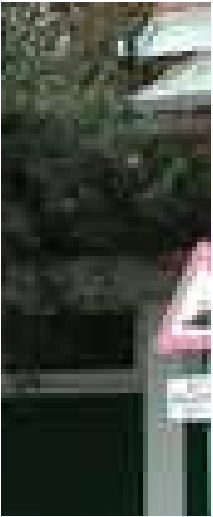
\includegraphics[height=2in]{../figures/examplePicture-crop.pdf} \label{fig:examplePicture}}
   \;
   \subfigure[features]{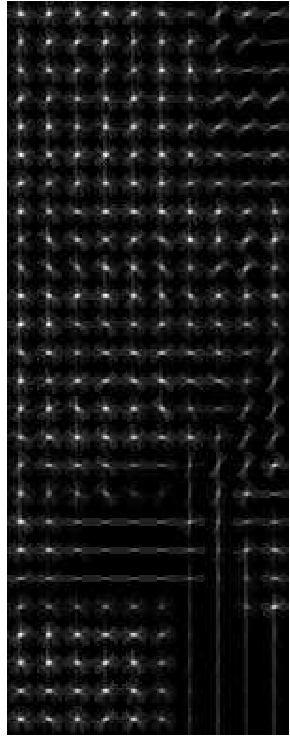
\includegraphics[height=2in]{../figures/exampleFeature-crop.pdf} \label{fig:exampleFeature}}
  \caption{Picture No 200 and features extracted form it, using Piotr's toolbox (http://vision.ucsd.edu/~pdollar/toolbox/doc/index.html) %TODO where put this reference?
  }
\end{figure}



% 
% TODO: test matrices descriptions.
% 
% \subsection*{Data analysis and preparation}
% We took a look at various distributions of the data and we have found out that:
% \begin{enumerate}[1.]
% \item Most of the artists have only few distinct listeners. (\ref{fig:artistListeners}). First, we have $1262$ artists for which there don't exist even a single listener, so we cannot predict anything reasonable for them. Then, $90.26\%$ of all the artists have at most $5$ different listeners.
% \begin{figure}[!t]
% \center
% \subfigure[Numbers of artists with various number of listeners. We see that most of the artists have only $1$ or $2$ listeners.]{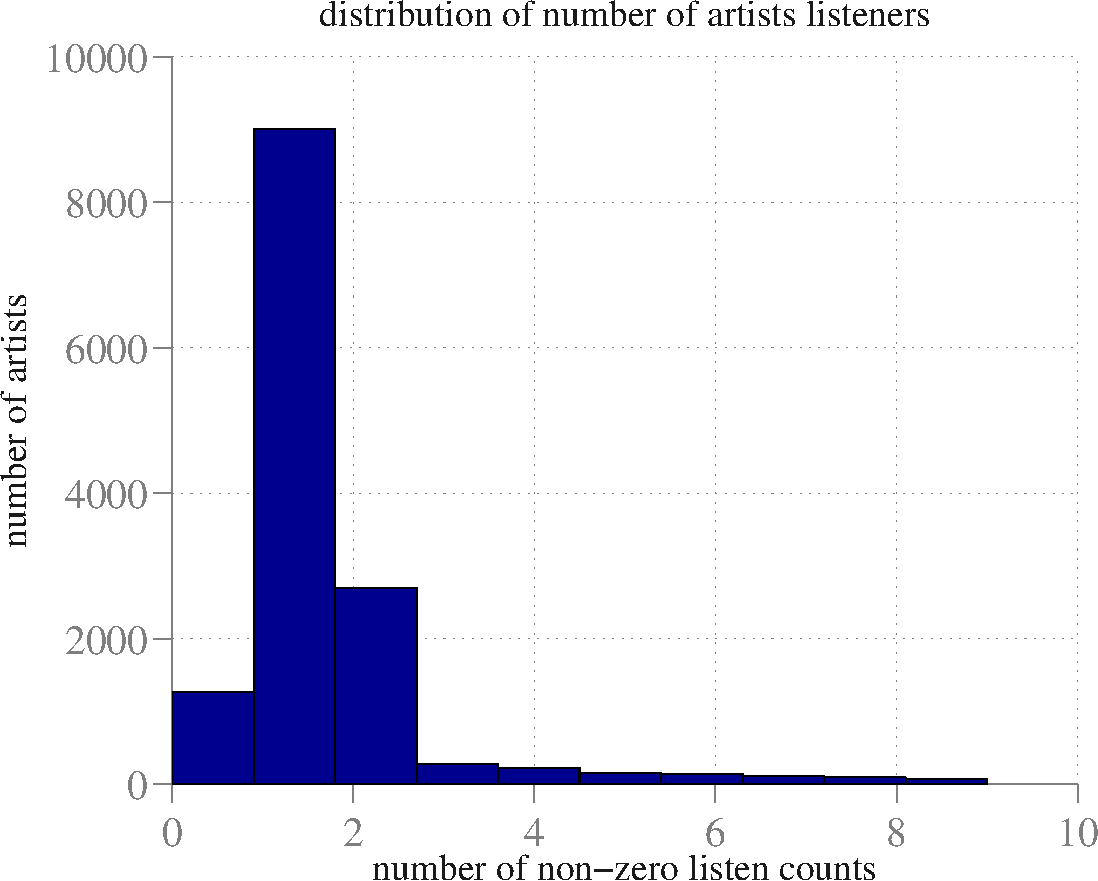
\includegraphics[width=2.5in]{../figures/artist_listeners_count-crop.pdf} \label{fig:artistListeners}}
% \hfill
% \subfigure[Number of artists for given value of standard deviation of listen counts of users (excluding zero standard deviation)]{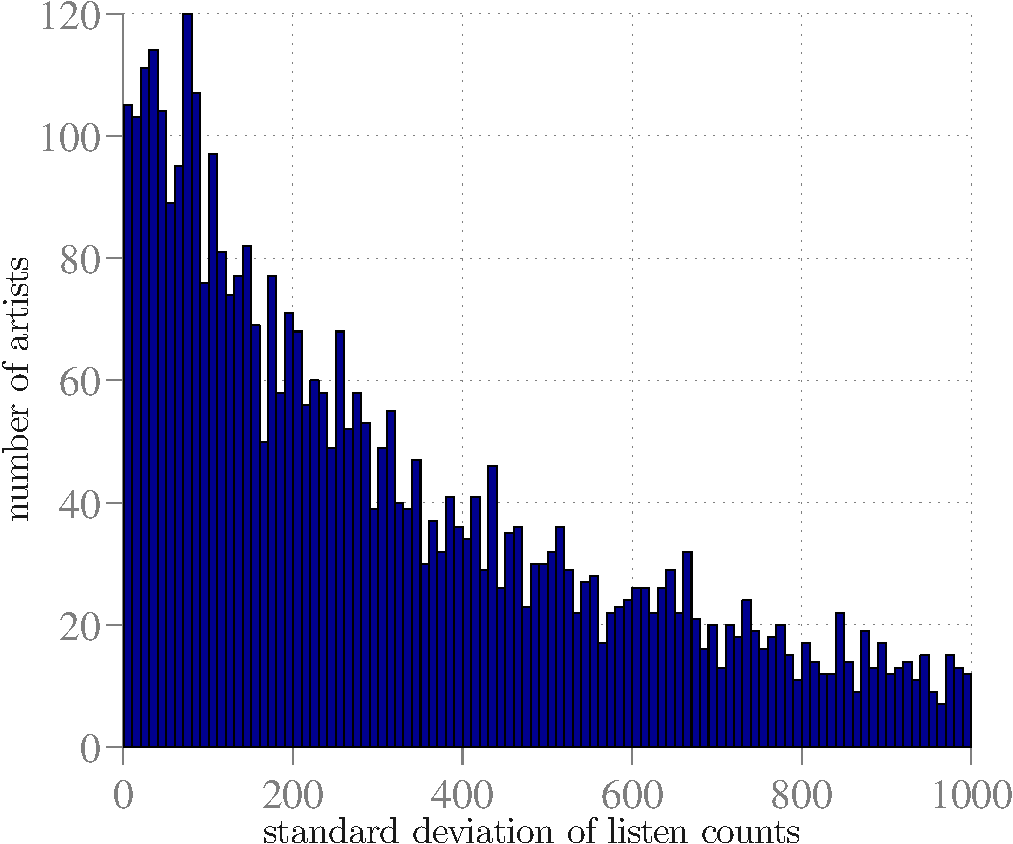
\includegraphics[width=2.5in]{../figures/artist_listeners_std-crop.pdf} \label{fig:artistListenersStd}}
% \caption{Analysis of listen counts for given artist}
% \end{figure}
% \item Among $4812$ artists, who have more than one listener, there is very big standard deviation of listen counts for different users: \ref{fig:artistListenersStd}. E.g. only $93$ of them have standard deviation of listen counts $<10$, and $1017$ have $\mbox{std} < 100$. From this we expect big errors in prediction as in most cases we will have very little data about given artist and the data we will be very uncertain.
% \item Distribution of all listen counts (for all artists and all users) is not Gaussian: \ref{fig:listenCounts}. It rather resembles $\frac{1}{x}$ or $e^{-x}$. We tried applying various transformations to normalize the data. We decided to use logarithm, which gave us effect shown on \ref{fig:logListenCounts}. Later, we normalized the data.
% %TODO: pisac o tym, ze artysci mieli dziure w sumie odsluchan? brac to pod uwage?
% \end{enumerate}
% 
% 
% \begin{figure}[!t]
% \center
% \subfigure[For each (user, artist) listen count value - how many times does it occur in $Y_{train}$ ]{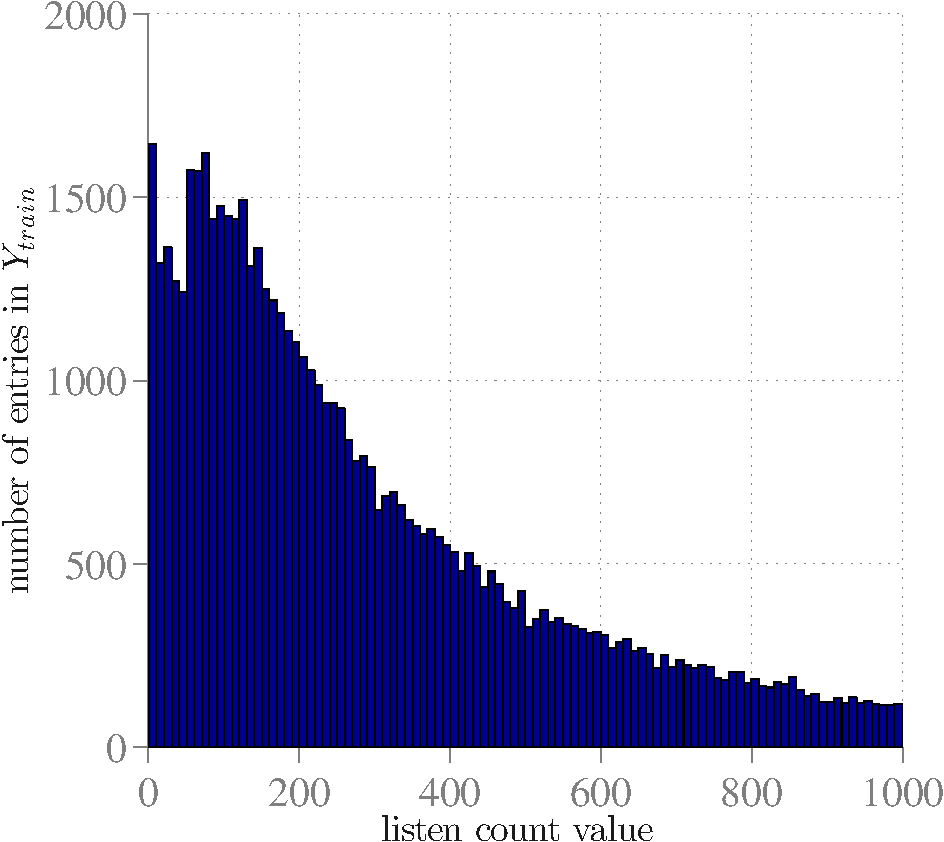
\includegraphics[width=2.5in]{../figures/listen_counts-crop.pdf} \label{fig:listenCounts}}
% \hfill
% \subfigure[Same histogram as in \ref{fig:listenCounts}, but after taking logarithm of each value]{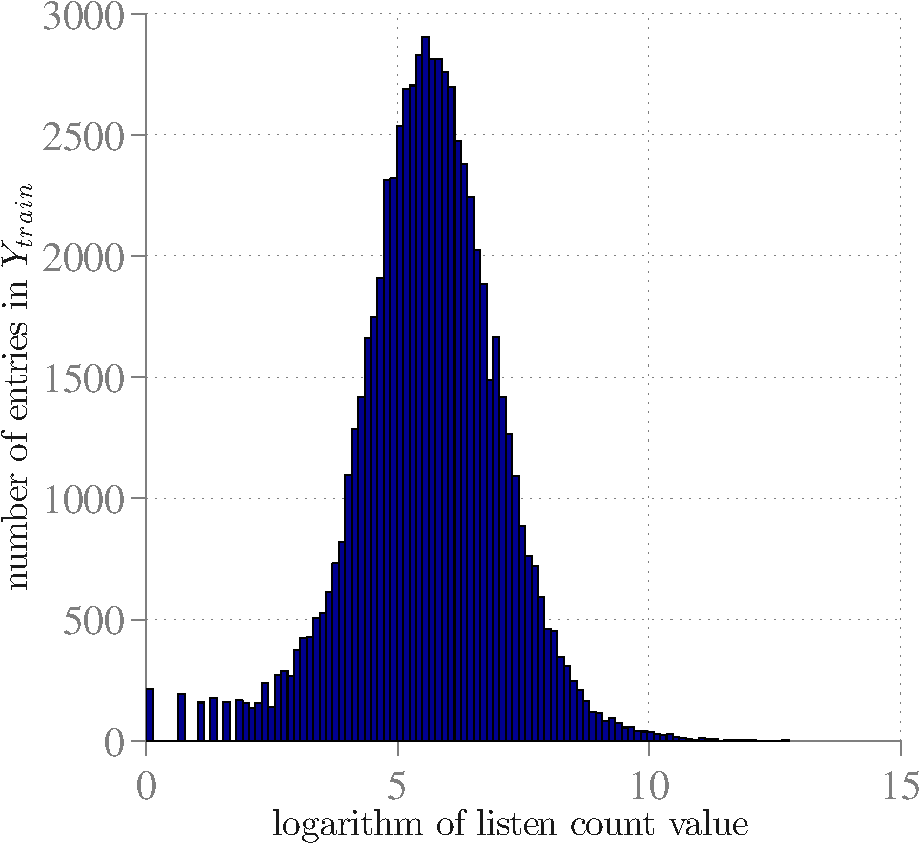
\includegraphics[width=2.5in]{../figures/log_listen_counts-crop.pdf} \label{fig:logListenCounts}}
% 
% \caption{Analysis of whole set of listen counts}
% \end{figure}

\end{document}
